\documentclass[a4paper,twoside,final]{article}
%----Eingebundene Bibliotheken-----
\usepackage[ngerman]{babel}         % Deutsches Sprachpaket
\usepackage[utf8]{inputenc}         % Eingaben codieren
\usepackage[T1]{fontenc}            % Umlaute codieren, Silbentrennung
\usepackage{amsmath, amssymb}       % Mathe
\usepackage{amsthm,amstext,amsxtra} % Symbole für Mathe
\usepackage{mathtools}              % \Aboxed Boxen in align
\usepackage{wrapfig}                % Bilder umfließen
\usepackage{svg}                    % Vektorgraphiken einbinden
\usepackage{geometry}               % Papierformat
\usepackage{tabularx}               % Tabellen
\usepackage{xcolor,colortbl}        % Farben
\usepackage{graphicx}               % Für Limes Definition wichtig
\usepackage{soul}                   % Unterstreichungen
\usepackage[section]{placeins}      % \Floatbarrier
\usepackage{wrapfig}                % Bilder umfließen
\usepackage{enumerate}              % Aufzählungen
\usepackage{footnote}               % Fußzeilen
\usepackage{booktabs}               % publication quality tables
\usepackage[hyphens]{url}           % \url{}
\usepackage{bm}                     % bold symbols \bm{r}
\usepackage{dsfont}                 % identity matrix \mathds{1}
\usepackage{enumitem}               % itemize Umgebungen customizen
\usepackage{esint}                  % Doppelintegrale
\usepackage{fancyhdr}               % schöne Kopf- und Fußzeilen
\usepackage{lmodern}
\usepackage{tikz}
\usepackage{pgfmath, pgfplots}
\usepackage[labelfont=bf]{subcaption}
\usepackage[square,numbers,sort&compress]{natbib}
\usepackage{mhchem}                 % Chemistry Package
\usepackage{physics}
\usepackage{chemfig}
\usepackage[detect-all,
            locale=DE,binary-units,
            exponent-product=\cdot
            ]{siunitx}              % \SI{12}{\gram}
%siunitx stellt für Tabellen den Spaltentyp S bereit ==> Ausrichtung an Dezimaltrennzeichen
\usepackage[position=below,
            tableposition=top,
            format=hang,
            labelfont=it,
            labelfont=bf,
            ]{caption}              % Settings für Captions
\captionsetup[wrapfigure]{name=Abb.}
\usepackage[europeanvoltages,
            europeancurrents,
            europeanresistors,
            americaninductors,
            europeanports
            ]{circuitikz}           % Schaltungen
\usepackage{chngcntr}               % vor hyperref laden!
  \counterwithin*{equation}{section}
  \counterwithin*{figure}{section}
  \counterwithin*{table}{section}

\usepackage[final,
            pdfauthor={Martin Beyer, Vanessa Huth},
            pdfsubject={Fortgeschrittenen-Praktikum},
            pdffitwindow=true,      % resize document window
            pdftitle={Fortgeschrittenen-Praktikum},
            bookmarks=true,         % lesezeichen-Liste
            bookmarksopen=true,     % Lesezeichen geöffnet
            bookmarksopenlevel=1,
            bookmarksnumbered=true,
            colorlinks=true,        % fuer Druckversion auf "false"
            linkcolor=blue,         % Table of Contents, Footnotes
            urlcolor=blue,          % fuer eingebunden URLs
            citecolor=blue,         % Equations, References
            filecolor=blue,
            pdfborder={0 0 0},      % keine Rahmen um Links: {0 0 0}
            ]{hyperref}


% Commands
\renewcommand{\sfdefault}{lmss}     % latin modern sans serif
\newcommand{\R}{\mathbb{R}}         % Reelle Zahlen
\newcommand{\N}{\mathbb{N}}         % Natürliche Zahlen
\newcommand{\C}{\mathbb{C}}         % Komplexe Zahlen
\newcommand{\de}{\mathrm{d}}      % Differential
\newcommand{\entspricht}{\mathrel{\widehat{=}}}

\DeclareSIUnit{\eV}{\text{eV}}
\DeclareSIUnit{\voltpeakpeak}{\volt{\textsubscript{pp}}}

% Dokumenteneinstellungen
\setlength{\parindent}{0px}         % remove indent in new paragraph
\setlength{\parindent}{0px}         % keine Absätze durch Leerzeilen im Code
\emergencystretch=1em % Definiert den Leerraum, der innerhalb einer Zeile zusätzlich verteilt werden darf.
\setlength{\topmargin}{-5mm} % 210mm = 8.2677165in
\newlength{\mylength}
\setlength{\mylength}{\paperwidth}
\addtolength{\mylength}{-2in} % standardmäßig wird den Seitenrändern jeweils noch 1in = 25.4mm hinzuaddiert
\setlength{\textwidth}{145mm}
\setlength{\textheight}{230mm}
\addtolength{\mylength}{-\textwidth}
\setlength{\oddsidemargin}{10mm}
\addtolength{\mylength}{-\oddsidemargin}
\setlength{\evensidemargin}{\mylength}
\setlength{\marginparwidth}{1.7cm}
\interfootnotelinepenalty=10000

% Umdefinition von \textcolor ********************************************************
\makeatletter
\renewcommand*{\@textcolor}[3]{%
	\protect\leavevmode
	\begingroup
	\color#1{#2}#3%
	\endgroup
}
\makeatother
% Damit das auch im Mathemodus anwendbar ist und dort z.B. die Leerzeichen nicht wie im Textmodus gesetzt werden.

\pgfplotsset
{compat=newest, % aktuelle Version: 1.16 [29.05.2018]
	/pgf/number format/.cd, % cd steht fuer current directory
	%  	use comma, % Komma als Dezimaltrennzeichen %%% UNCOMMENT THIS !!!
	1000 sep={} % Legt das Tausendertrennzeichen fest
}
%\usepgfplotslibrary{external} % Section 7.1.1 Using the Automatic Externalization Framework of TikZ
%\tikzexternalize[prefix=FiguresTikZ/] % activate externalization! Use subdirectory [FiguresTikZ]
\usepgfplotslibrary{fillbetween}
\usepgfplotslibrary{polar}
\usetikzlibrary{arrows.meta}
\usetikzlibrary{calc}
\usetikzlibrary{datavisualization.formats.functions}
\usetikzlibrary{intersections}
\usetikzlibrary{patterns}
\usetikzlibrary{pgfplots.colormaps}
\usetikzlibrary{plotmarks}
\usetikzlibrary{shapes.geometric}

% Generelle Festlegung des Styles fuer Blockschemata (Plaene fuer Regelkreise, etc.)
\tikzstyle{block} = [draw, fill=blue!20, rectangle, minimum height=1cm, minimum width=1cm]%, minimum width=6em]
\tikzstyle{sum} = [draw, fill=blue!20, circle, node distance=1cm]
\tikzstyle{input} = [coordinate]
\tikzstyle{output} = [coordinate]
\tikzstyle{pinstyle} = [pin edge={to-,thin,black}]

\begin{document}
\setlength{\marginparsep}{2em}
\renewcommand{\theequation}{\arabic{section}.\arabic{equation}}
\renewcommand{\thefigure}{\arabic{section}.\arabic{figure}}
\renewcommand{\thetable}{\arabic{section}.\arabic{table}}

% Anfang ********************************************************
\begin{center}
\thispagestyle{empty}
  
\includegraphics[width=0.75\textwidth]{../UniJena_BildWortMarke_black.pdf}\\[4em]
  \Large
  Ausarbeitung zum Versuch\\[2em]
  \Huge
  Rastersondenmikroskopie\\
  \vspace{2cm}
  \Large
  Martin Beyer und Vanessa Huth\\[2em]
  Abgabe: 21. Januar 2020\\[2em]
  Betreuer: Dr. Marco Grünewald\\[5em]
  \begin{flushleft}
  	Bewertung und Ausarbeitung:\\[2em]
		Protokollführung und Form:\\[1em]
		Ergebnisse, Auswertung und Interpretation:\\[1em]
		Bemerkungen und Hinweise des Betreuers:
  \end{flushleft}
\end{center}
\clearpage

\pagestyle{fancy}
\renewcommand{\headrulewidth}{0pt}
\renewcommand{\footrulewidth}{0.5pt}
\renewcommand{\sectionmark}[1]{\markright{#1}}
\fancyhead[RO,LE]{\textbf{Rastersondenmikroskopie}}
\fancyhead[RE,LO]{\rightmark}
\fancyfoot[LE,RO]{\bfseries\thepage}
\fancyfoot[CO,CE]{Protokoll}
\renewcommand{\headrulewidth}{0.5pt}
\renewcommand{\footrulewidth}{0.5pt}

\setcounter{equation}{0}
\setcounter{figure}{0}

% *********************************************
% ***** KAPITEL 1 *****************************
% *********************************************
\tableofcontents
% \pagenumbering{gobble}% remove page numbering
\newpage
% \pagenumbering{arabic}
\section{Aufgabenstellung} \label{sec:Aufgabenstellung}
\paragraph*{Präparation von Tunnelspitzen}$~$\\
Es erfolgt eine Herstellung der Tunnelspitzen nach der in~\cite{Nanosurf} beschriebenen Anleitung durch Abschneiden.
\subsection{Untersuchung polykristalliner Goldoberflächen}
Es werden reproduzierbare Bilder mehrerer Vergrößerungsstufen aufgenommen und eine Optimierung der mikroskopischen Auflösung und Abbildungsqualität durchgeführt. Dabei werden insbesondere die Tunnelparameter, Regelkreisparameter und Abtastgeschwindigkeit variiert. Es erfolgt eine geeignete Darstelunng der mikroskopischen Aufnahmen vor und nach der Bildbearbeitung.\\
Weiterhin wird die Probenoberfläche quantitativ und qualitativ charakterisiert, indem die Rauheit, Kristallitgrößen, -durchmesser und -höhen ausgemessen werden.
\subsection{Untersuchung verschiedener Proben}
Analog zur Goldoberfläche wird die Bildaufnahme optimiert und Probenparameter charakterisiert. Es werden folgende Proben untersucht:
\begin{itemize}
  \item Einkristallines Graphen auf Siliziumkarbid:
  \begin{enumerate}
    \item Dabei soll atomare Auflösung erreicht werden und auftretende Probleme diskutiert und der Einfluss der Tunnelspannung untersucht werden.
    \item Die Atomabstände und Stufenhöhen im Graphen werden ausgemessen und durch FFT ausgewertet.
  \end{enumerate}
  \item Kohlenstoffnanoröhren auf graphitisierten Siliziumkarbid werden untersucht und charakterisiert. Probleme bei der Aufnahme sollen diskutiert werden.
  \item Durch Vakuumbedampfung werden eigene Metallschichten hergestellt und untersucht.
\end{itemize}

\paragraph{Erklären von Abbildungsfehlern}$~$\\
Typisch auftretende Abbildungsfehler, welche durch Spitze, Piezoscanner, Elektronik, Regelkreis, äußere Störungen, oder Software verursacht werden, sollen erkannt und anhand von Beispielen der eiegenen Messung beschrieben und erklärt werden.

\paragraph{Bildbearbeitung mit Gwyddion}$~$\\
Das Programm Gwyddion~\cite{Gwyddion} wird zur Kontrastierung und Untergrundkorrektur benutzt. Es erfolgt eine Bildbearbeitung mit einer zweidimensionalen Fast Fourier Transformation (FFT).\\
Weiterhinn können Filter eingestellt, Glättung durchgeführt und Probenparameter (Gitterkonstanten, Stufenhöhen, Rauheit) bestimmt werden.

% *********************************************
% ***** KAPITEL 2 *****************************
% *********************************************
\newpage
\section{Grundlagen} \label{sec:Grundlagen}
\subsection{Rastertunnelmikroskop}
\subsubsection{Aufbau und Funktionsweise}\label{sec:STM_Aufbau}
Bei einem Rastertunnelmikroskop STM (\textit{Scanning Transmission Microscope}) wird eine idealerweise einatomar dünne metallische Spitze als Sonde zur Abrasterung einer elektrisch leitfähigen Probe benutzt. Dabei wird die Tunnelspitze auf etwas \SI{1}{\nano\metre} an die Oberfläche herangeführt, bis bei einer angelegten Spannung ein elektrischer Tunnelstrom fließt~\cite{Versuchsanleitung}. Nachdem ein Tunnelkontakt hergestellt wurde, wird die Spitze durch eine Rastereinheit bestehend aus piezoelektrischen Stellelementen rasterförmig über einen kleinen Bereich von wenigen \si{\nano\metre} bis \si{\micro\metre} über die Probe bewegt. Der fließende Strom $I_T$ ist dabei abhängig von der angelegten Vorspannung und der elektrischen Zustandsdichte $\rho$ der Probe und Tunnelspitze bei der Fermienergie $E_F$. Es ergibt sich folgender Zusammenhang:
\begin{align}
  I_T \propto \int_{E_F}^{E_F+ eU_V} \rho_\text{Spitze}(E_F)\;\rho_\text{Probe}(E_F+eU_V) \;T(E,U_V)\,\de E.\label{eqn:Tunnelstrom}
\end{align}
Bei $T$ handelt es sich um einen Transmissionskoeffizienten, der von der Energie und Vorspannung abhängt. Für kleine Spannungen bildet das Rastertunnelmikroskop die elektronische Zustandsdichte der Oberfläche nahe der Fermienergie ab. Daraus lässt sich folgern, dass die Aufnahme eines STM nicht die Atome direkt, sondern die an die Atome gebundenen Zustände abbildet.\\
Die Zustandsdichte der Oberflächenzustande fällt exponentiell mit der inversen Abfallslänge $\kappa$ ab, woraus ein exponentieller Abfall des Tunnelstroms mit wachsendem Proben-Spitzen Abstand $d$ resultiert
\begin{align}
  I \propto \exp(-2\kappa d).
\end{align}
Die exponentielle Spannungs-Strom Abhängigkeit ist wesentlich für eine präzise Messgenauigkeit des Rastertunnelmikroskops.\\
Der schematische Aufbau eines STM ist in Abbildung~\ref{fig:Rastertunnelmikroskop} dargestellt. Dabei wird die Spitze meist zusätzlich noch mit einem PID-Regelkreis angesteuert, um den Spitzen-Proben Abstand zu regeln.
\begin{figure}[htp]
    \centering
    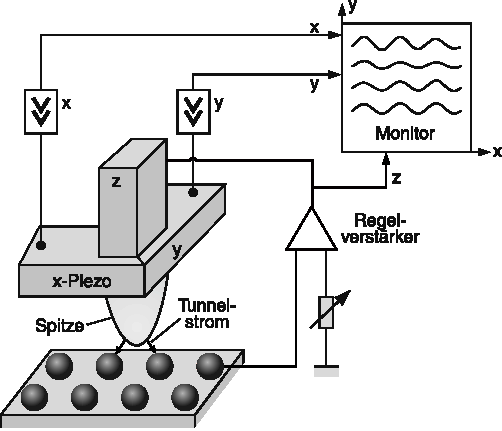
\includegraphics[width=0.5\textwidth]{Bilder/Raster_Tunnelmikroskop.pdf}
    \caption{Schematischer Aufbau eines Rastertunnelmikroskops aus~\cite{Demtroeder}.}
    \label{fig:Rastertunnelmikroskop}
\end{figure}

\subsubsection{Tunneleffekt}
Um das auftreten des Tunnelstroms zu erklären, muss analysiert werden, wie Ladungsträger von besetzten Zuständen einer Elektrode durch einen Potentialwall in die unbesetzten Zustände einer zweiten Elektrode gelangen können. Im Rahmen der klassischen Physik kann ein Teilchen diesen Potentialwall nur überwinden, wenn seine Energie $E$ größer als das Maximum des Potentialwalls ist. Laut der Quantenmechanik ist ein Elektron mithilfe einer Wellenfunktion $\Psi(x)$ beschreibbar, dessen Verlauf im eindimensionalen Fall in Abbildung~\ref{fig:Tunneleffekt} gezeigt wird.
\begin{figure}[htp]
    \centering
    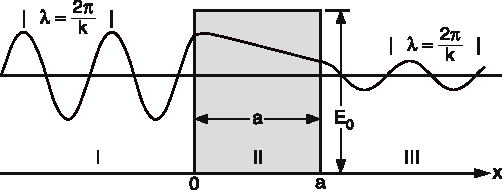
\includegraphics[width=0.7\textwidth]{Bilder/Tunneleffekt.pdf}
    \caption{Quantenmechanischer Tunnelffekt an einer rechteckigen Potentialbarriere der Höhe $E_0$ aus~\cite{Demtroeder}}
    \label{fig:Tunneleffekt}
\end{figure}
Für dieses zeitunabhängige Problem $\Psi(x,t) = \Phi(x)\cdot\exp(-iEt/\hbar)$ gehorcht das Elektron der stationären Schrödingergleichung
\begin{align}
  E \Psi(x) = \left[-\frac{\hbar^2}{2m_e}\Delta + V(x)\right] \Psi(x),
\end{align}
welche eine Differentialgleichung für den harmonischen Oszillator darstellt mit der Lösung
\begin{align}
  \Psi(x) = A_1 \exp(ikx) + A_2 \exp(-ikx), \quad k=\sqrt{\frac{2m(E-V)}{\hbar^2}}.
\end{align}
Im Bereich II ergibt sich mit $E_0 > E$ ein exponentiell abfallender Verlauf der Wellenfunktion. Jedoch verschwindet die Wellenfunktion im Bereich III nicht, sodass das Elektron mit endlicher Wahrscheinlichkeit durch den Potentialwall in die Probe tunneln kann. Im Mittel tunneln jedoch Elektronen auch zu gleicher Anzahl von der Probe in die Spitze, sodass kein Nettostrom messbar ist. Wird nun noch eine Spannung zwischen Spitze (I) und Probe (III) angelegt, dann ergibt sich der in Abbildung~\ref{fig:Tunneleffekt_Spannung} dargestellte Potentialverlauf. Die Energieniveaus der Tunnelspitze liegen nun höher und es bildet sich eine Vorzugsrichtung des Tunneleffektes aus. Hierbei fließt nun ein Tunnelstrom von der Probe zur Spitze.
\begin{figure}[htp]
    \centering
    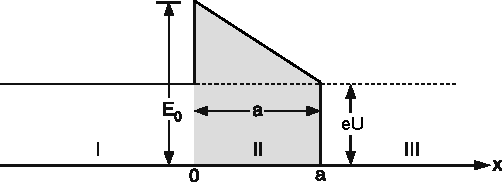
\includegraphics[width=0.7\textwidth]{Bilder/Tunneleffekt_Spannung.pdf}
    \caption{Potentialverlauf zwischen Spitze (I) und Probe (III) bei angelegter Spannung $U$ nach~\cite{Hamann} (eigene Abbildung)}
    \label{fig:Tunneleffekt_Spannung}
\end{figure}

\subsubsection{Betriebsarten}
Es gibt prinzipiell zwei verschiedene Arten, ein Rastertunnelmikroskop zu betreiben. Je nach Art und Struktur der Probe bieten diese jeweils Vorteile.
\paragraph{Konstante Höhe} Am leichtesten lässt sich das Tunnelbild realisieren, indem die Variation des Tunnelstroms direkt als Funktion des Ortes gemessen wird, wobei die Spitze auf konstanter Höhe verweilt. Dabei ergibt sich ein Strombild. Das Verfahren hat den Vorteil, dass die Probe besonders schnell abgerastert werden kann und die Höhe der Spitze nicht mithilfe eines Regelkreises gesteuert werden muss. Allerdings eignet sich das Verfahren nur für flache Proben, da sonst die Spitze mit der Probe kollidieren kann. Eine Kollision stellt dabei eine starke Wechselwirkung mit der Probe dar, welche die Spitze verformt oder der direkte mechanische Kontakt.
\paragraph{Konstanter Strom} Meist ist es jedoch vorteilhafter auf das langsamere Verfahren des konstanten Stroms zurückzugreifen. Hierbei wird ein Piezoelelement der Spitze mit einem PID-Regelkreis verbunden, der dafür sorgt, dass der fließende Strom konstant gehalten wird. Dabei wird die Variation der exponentiell zum Abstand abfallenden Zustandsdichte der Probenoberfläche gemessen. Das resultierende Bild entspricht also einer Fläche konstanter Zustandsdichte der Probe. Je nach Geschwindigkeit des Regelkreises kann dies allerdings dazu führen, dass scharfe Kanten der Probe durch die Spitze nicht registriert werden. Dies wird am Spitzenverlauf in Abbildung~\ref{fig:Betriebsmodi} ersichtlich. Da bei diesem Verfahren die Höhe der Spitze ständig angepasst wird, ist sie auch für raue Proben geeignet, allerdings aufgrund der Regelzeit entsprechend langsamer.
\begin{figure}[htp]
    \centering
    \begin{subfigure}{0.45\textwidth}
        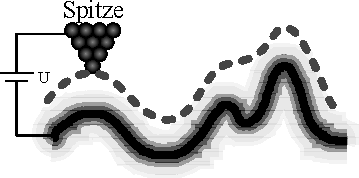
\includegraphics{Bilder/STM_konstStrom.pdf}
        \caption{Konstanter Strom}
    \end{subfigure}
    \hspace{1cm}
    \begin{subfigure}{0.45\textwidth}
        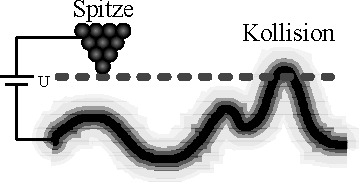
\includegraphics{Bilder/STM_konstHoehe.pdf}
        \caption{Konstante Höhe}
    \end{subfigure}
    \caption{Darstellung der beiden Betriebsmodi eines STM.}
    \label{fig:Betriebsmodi}
\end{figure}

\subsubsection{PID-Regelkreis}
Ein Regelkreis stellt einen Wirkungsablauf zur Beeinflussung einer physikalischen Größe in einem technischen Prozess dar. Dabei wird der aktuelle Wert an den Regler zurückgeführt und mit einer Führungsgröße, dem Sollwert verglichen. In diesem Experiment soll der Tunnelstrom geregelt werden. Der Regler wirkt der Abweichung entgegen und besteht aus verschiedenen Gliedern die im Schema~\ref{fig:PID} zusammengefasst sind.
\begin{figure}[htp]
    \centering
    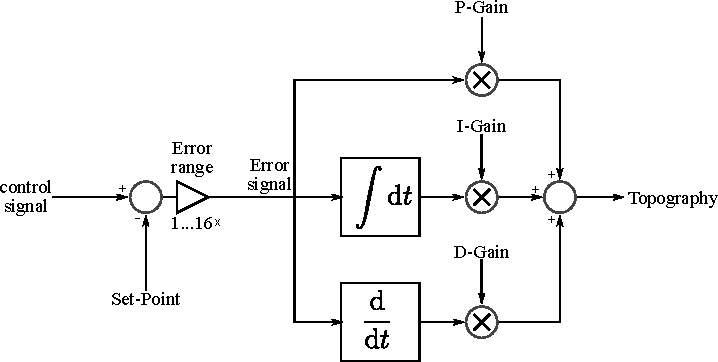
\includegraphics[width=0.7\textwidth]{Bilder/PID-Regler.pdf}
    \caption{Schematischer Aufbau des verwendeten PID-Regelkreises nach~\cite{Versuchsanleitung}.}
    \label{fig:PID}
\end{figure}\\
Heutzutage wird hauptsächlich eine Kombination von Proportional-, Integral- und Differenzialregler verwendet und unter dem Begriff des PID-Reglers zusammengefasst.
\paragraph{Proportionalregler} Das P-Glied besteht aus einem proportionalen Anteil mit der Verstärkung $K_P$. Als Regler eingesetzt multipliziert es die Regelabweichung mit seinem Verstärkungsfaktor $K_P$ und gibt das Ergebnis weiter. Ein P-Regler allein kann eine Regelabweichung nicht beheben.
\paragraph{Integralregler} Das I-Glied besitzt ein integratives Verhalten, denn es summiert die Regelabweichung zeitlich auf und multipliziert die Summe mit dem Faktor $K_I$. Je länge die Regelabweichung anhält, desto größer wird die Stellgröße des I-Gliedes.
\paragraph{Differenzialregler} Das D-Glied besitzt ein differentielles Verhalten, es bewertet die Änderung der Regelabweichung und berechnet die Änderungsgeschwindigkeit, welche mit dem Faktor $K_D$ multipliziert wird. Das D-Glied kann durch die Bildung der Ableitung den Verlauf des Signals \glqq vorhersagen\grqq, ist allerdings wirkungslos, wenn sich die Abweichung nicht ändert.\\
Ein PID-Regler ist geeignet, um den Tunnelstrom während einer STM-Messung konstant zu halten. In seiner Gesamtheit wirkt ein PID-Regler außerdem als ein Tiefpass und kann dazu eingesetzt werden, Rauschsignale zu filtern. Durch Anpassung der verschiedenen Faktoren kann die Regelgeschwindigkeit optimiert werden.
\subsection{Rasterkraftmiskroskop}
Das Kernstück des Rasterkraftmikroskop (RKM, englisch auch Atomic Force Microscope (AFM)) ist im Wesentlichen identisch zu dem des Rastertunnelmiskroskops. Auch hier wird eine feine Spitze verwendet, welche in einem charakteristisch kleinem Abstand gegenüber der Probe über diese gerastert wird. Die Höhe der Spitze über der Probe wird in beiden Fällen durch piezoelektrische Stellelemente realisiert. \\
Der Unterschied zwischen beiden Miksrokopiearten besteht in der vorrausgesetzen Probeneigenschaften. Während beim Rastertunnelmiskroskop, da hier ein elektrischer Tunnelstrom gemessen wird, ausschließlich leitende Proben verwendet werden können, sind für Messungen mit dem Rasterkraftmikroskop auch Isolatoren geeignet.

\subsubsection{Aufbau}
Die Besonderheit im Aufbau des RKM liegt darin, dass hier die Spitze auf eine Blattfeder montiert ist. Das Gebilde aus Blattfeder und Spitze wird Cantilever genannt. Je nach Modi wird die Spitzen-Blattfeder-Konstruktion auf unterschiedliche Weise über die Probe gerastert.

\subsubsection{unterschiedliche Messmodi}
Beim RKM werden grundsätzlich 3 verschiedene Messmodi unterschieden.
\subparagraph{Kontaktmodus}
Die feine Spitze wird in diesem Messmodus mit Federkraft auf die Probe gedrückt, steht also in direktem mechanischem Kontakt zur Oberfläche. \\
Erfolgt die Messung nach der \textbf{constant height method}, hält die Spitze eine konstante Höhe in z-Richtung. Die Abtastnadel verbiegt sich hierbei entsprechend der Oberfläche. Diese Messmethode findet auch beim RTM Anwendung. \\
Die \textbf{constant force method} ist entsprechend der constant current method beim RTM und unterscheidet sich nur in der gemessenen Größe, welche konstant gehalten wird. Bei der constant force method wird der Cantilever mittels eines piezoelektrischen Steuerelements so über die Probe gerastert, dass die Auslenkung des Cantilevers und damit die Kraft zwischen Spitze und Probe gleich bleibt. Das Auslenkungssignal der Blattfeder wird hierbei als Regelgröße in einen Regelkreis gegeben, der anschließend die Höhe der Spitze anpasst.\\
Vor- und Nachteile dieser Methoden sind identisch zu den äquivalenten Methoden beim RTM \ref{}.

\paragraph{Nicht-Kontaktmodus}
Beim Nicht-Konktaktmodus berührt die Spitze die Probe nicht. Der Cantilever wird hierbei mit der Schwingungsfrequenz $\omega_N$ zum Schwingen angeregt. Beim Schweben der Spitze über die Probe kommt es zu anziehenden Kräften zwischen Spitze und Oberfläche. Meist handelt es sich um Van der Waals Kräfte, je nach Spitzenmaterial können aber auch elektrische oder magnetische Kräfte auftreten. Die Kräfte beeinflussen die Resonanzfrequenz der Feder und die darausfolgendde Änderung wird gemessen.

\paragraph{Tappping Modus}
Auch bei diesem Messmodus wird die Spitze zu Schwingungen angeregt, tippt die Oberfläche aber bei ihren Schwnigungen leicht an.

\subsection{Weitere Rastersondenmikroskope}
Mit dem Magnetkraftmikroskop gelingt es die lokale Magnetstärke in der Probe zu untersuchen. Hierbei ist die Abstastnadel mit einem ferromagnetischen Material beschichtet. Die Messung für jede Bildzeile erfolgt in zwei Durchläufen. Im ersten Durchgang wird mittels eines der vorher beschriebenen Messmodi das Höhenprofil aufgenommen. Im zweiten Durchgang wird die Messnadel mit konstantem Abstand über die Oberfläche gerastert.\\

Zusätzlich gibt es noch weitere Rastersondenmikroskope, die die Wechselwirkung zwischen Sonde und Probe nutzen und die die Probe Punkt für Punkt abtasten. Das Grundprinzip aller ist dabei gleich des oben beschriebenen, sie unterscheiden sich im Wesentlichen durch die Abstastung anderer Probeneigenschaften. Dazu zählen zum Beispiel das Optische Rasternahfeldmikroskop (engl. Scanning Nearfiel Optical Microscope, kurz SNOM), das Rasterelektronenmikroskop (REM, engl. SEM) sowie das akustische Rasternahfeldmikroskop (ARNM, engl. scanning near-field acoustic microscope (SNAM).

\subsection{Piezoeffekt und piezoelektrische Stellelemente}
Für die Bedienung und Funktionsweise der Rastersondenmikroskope ist das Einstellen der Position der Sonde im Subnanometerbereich von entscheidender Bedeutung. Dies wird durch piezoelektrische Stellelemente realisiert. Hierbei wird der \textit{(inverse) piezoelektrische Effekt} genutzt.
\paragraph{Piezoelektrischer Effekt} Wird Druck auf einen piezoelektrischen Kristall ausgeübt, kommt es zur Dipolbildung in der Elementarzelle und makroskopisch ist eine elektrische Spannung messbar. Ein Jahr nach der Endeckung des piezoelektrischen Effekts 1880 fanden dessen Entdecker Jaques und Pierre Curie auch den inversen piezoelektrischen Effekt: Wird ein elektrisches Feld angelegt, verformt sich der Kristall. Diese Eigenschaft wird in piezoelektrischen Stellelementen genutzt~\cite{Versuchsanleitung}.
\paragraph{piezoelektrische Stellelemente}
Häufig verwendete Bauformen piezoelektrischer Stellelemente sind Rohraktoren, Stapeltranslatoren und Streifenaktoren.
\textit{Rohraktoren} sind monolithische Keramikrohre, die innen und außen mit Elektroden beschichtet sind. Sind die Außenelektroden in vier \SI{90}{\degree} Segmente geteilt,  bewirkt eine differentielle Ansteuerung gegenüberliegender Elektroden eine Verbiegung des Rohrs. Diese Bauform findet häufig Einsatz als XY-Stelleinheit in Rastersondenmiskroskopen.
Stapeltranslatoren sind Linearaktoren und bestehen aus Stapeln von Keramikscheiben, zwischen denen sich Elektroden befinden. Bei Streifenaktoren handelt es sich um Konktraktoren. Sie bestehen aus dünnen laminierten Keramikstreifen und nutzen die Auslenkung orthogonal zur Richtung des elektrischen Feldes.\\
Piezoeelemente bieten Vorteile gegenüber mechanischen Stellelementen, denn sie können sehr robust gebaut werden und unterliegen werder Reibung noch Verschleiß. Meist weisen sie eine hohe Langzeitstabilität auf und sind einfach herstellbar~\cite{Versuchsanleitung}.
\newpage
\begin{wrapfigure}{r}{5.6cm}
  \centering
  \vspace{-3mm}
  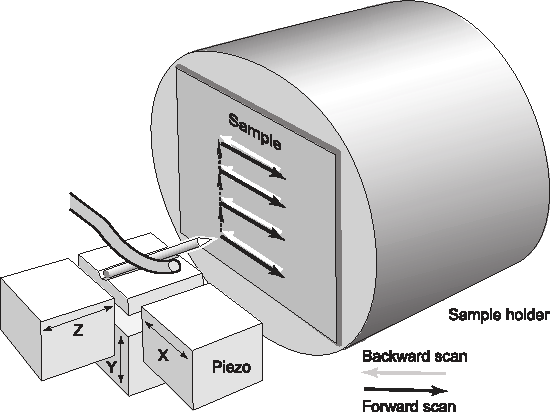
\includegraphics[width=5.4cm]{Bilder/Piezoscanner.pdf}
  \caption{Darstellung der Piezoscanneinheit~\cite{Nanosurf}}
  \label{fig:Piezo}
\end{wrapfigure}\\
Im Praktikum wird die in Abbildung~\ref{fig:Piezo} dargestellte Piezoeinheit verwendet. Unter Nutzung des inversen piezoelektrischen Effekts wird der \textit{Sampleholder} schrittweise an die Probe angenähert und während der Messung durch die $x$- und $y$-Piezos horizontal zur Spitze bewegt. Dadurch können Auflösungen im Ångström-Bereich erzielt werden.\\
Trotz ihrer hohen Stellgenauigkeit treten bei Piezoelementen Fehler auf. Zunächst zeigen sie meist eine nichtlineare Temperaturabhängigkeit und unterliegen der Hysterese. Dies bedeutet, dass die Verformung des Kristalls gegenüber der Spannungsänderung zeitverzögert verläuft~\cite{Versuchsanleitung}.

% *********************************************
% ***** KAPITEL 3 *****************************
% *********************************************
\section{Messapparatur und Versuchsdurchführung} \label{sec:Versuchsdurchführung}
\subsection{Versuchsaufbau und Spitzenpräparation}
Die Umsetzung eines SPM-Messsystems gestaltet sich als sehr übersichtlich. Die zwei grundlegenden Instrumente stellen der easyScan Scankopf und der Controller dar (Abbildung~\ref{fig:Messsystem}).\\
\begin{figure}[htp]
  \vspace{-5mm}
    \centering
    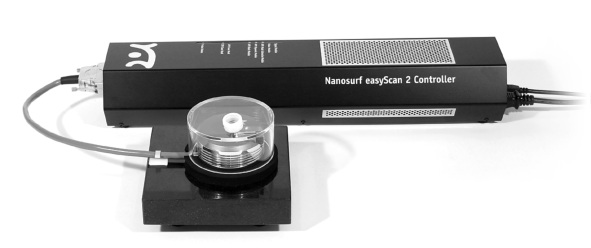
\includegraphics[width=0.7\textwidth]{Bilder/EasyScanSystem.pdf}
    \caption{Darstellung des Controllers und Scankopfes von Nanosurf easyScan}
    \label{fig:Messsystem}
\end{figure}\\
Zur Abrasterung der Probe wird ein Draht aus einer Platin-Iridium Legierung verwendet. Die Probe wird mit einer Piezoscanneinheit entlang der Probe geführt und an den Scankopf angenähert.
\begin{wrapfigure}{r}{5.6cm}
  \centering
  \vspace{-5mm}
  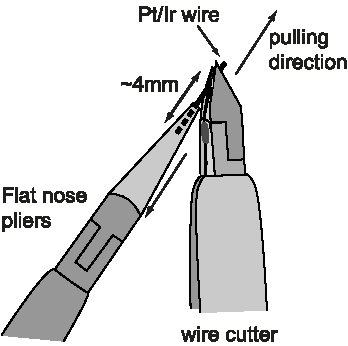
\includegraphics[width=5.5cm]{Bilder/WireCutter.pdf}
  \caption{Vorgehensweise zur Präparation der Messspitze}
  \label{fig:Spitzenpräparation}
\end{wrapfigure}
Die Probe ist auf einer metallischen Kreisscheibe mithilfe eines Silberleitlackes aufgeklebt. Das Scheibchen wird nun magnetisch an der motorgesteuerten Piezoeinheit angebracht und dies manuell auf wenige Millimeter an die Probe herangeschoben.
Der gesamte Scankopf steht auf einem separaten Tisch und steht auf einer kleinen Plattform, die Vibrationen dämpft. Zusätzlich befindet sich das Messsystem in einem großen mit Schaumstoff ausgekleideten Kasten.\\
Der Controller befindet sich außerhalb des Kastens und regelt die elektrische Ansteuerung der Probe, zudem zeigt er mithilfe einer LED den Status der Probe an.\\
Die Präparation der Spitze erfolgt nun mithilfe einer Pinzette und eines Seitenschneiders. Das hintere Stück des Drahtes wird mit der Pinzette gehalten und die Spitze mithilfe in einem schrägen Winkel abgeschnitten. Damit sich eine möglichst scharfe Spitze ergibt sollte diese eher durch Ziehen abgerissen werden, anstatt sie direkt durchzuschneiden. Die Vorgehensweise wird in Abbildung~\ref{fig:Spitzenpräparation} nochmal verdeutlicht. Die verwendete Spitze sollte an der Luft nicht oxidieren und zudem stabil und gleichzeitig elektrisch leitfähig sein. Aus diesem Grund werden Platinspitzen verwendet, wo Iridium zugesetzt wird. Chemisch geätzte Wolframspitzen weisen eine bessere Qualität auf, allerdings müssen diese im Hochvakuum verwendet werden, da sie sonst oxidieren.
%%% To Do: Messapparatur beschreiben
%%% To Do: Spitzenpräparation (Vergleich mit Wolframspitzen)
\subsection{Herstellung einer Probe mittels Vakuumbedampfung}
Im Verlauf des Versuchs soll ebenfalls die Herstellung einer eigenen Gold- oder Silberprobe mittels Bedampfung durchgeführt werden.\\
Dafür wird eine röhrenförmige, evakuierbare Kammer genutzt, wo eine bestimmte Menge des zu verdampfenden Materials auf ein Wolframschiffchen plaziert wird. Um bei der Bedampfung eine möglichst große freie Weglänge des verdampften Materials wird der Innenraum mithilfe einer Vakkuumpumpe auf einen Druck von $p = \SI{e-6}{\milli\bar}$ evakuiert.\\
Das zu bedampfende Plättchen wird magnetisch an einer Halterung an der Unterseite des Deckels befestigt. Während der Bedampfung wird durch einen starken Stromfluss durch das Wolframschiffchen das Metall komplett verdampft und verteilt sich im gesamten oberen Halbraum. Um die Menge an zu verdampfenden Materials zu berechnen, wird eine einfache Lambert-Verteilung herangezogen:
\begin{align}
  D(\vartheta) = D_\text{max} \cos\vartheta,
\end{align}
welche die Schichtdicke als Funktion des Polarwinkels $\vartheta$ bezüglich der senkrechten Achse beschreibt.\\
Um nun für eine gegebene aufzudampfende Schichtdicke $D \approx \SI{20}{\nano\metre}$ auf das Plättchen die Länge des Drahtes zu ermitteln, wird das Verdampfte Volumen in Beziehung zur Abhängigkeit der Lambert-Verteilung gesetzt
\begin{align}
  \de V = D(\vartheta)\de A = D_\text{max}\cos\vartheta\cdot h^2 \sin\vartheta \de \varphi\,\de\vartheta,
\end{align}
wobei $h \approx \SI{8}{\centi\metre}$ den vertikalen Abstand des Wolframschiffchens zum Plättchen beschreibt.
\begin{align}
  V_\text{Probe} &= V_\text{Draht} \frac{\displaystyle\int_{\varphi=0}^{2\pi}\int_{\vartheta'=0}^\vartheta D_\text{max}\cos\vartheta' h^2 \sin\vartheta'\; \de \vartheta'\,\de\varphi}{\displaystyle\int_{\varphi=0}^{2\pi}\int_{\vartheta'=0}^{\pi/2} D_\text{max}\cos\vartheta' h^2 \sin\vartheta'\; \de \vartheta'\,\de\varphi}.
  \intertext{Unter der Annahme eines zylindrischen Metalldrahtes $V_\text{Draht}=\pi\frac{d^2}{4}L$ mit $d\approx\SI{0.2}{\milli\metre}$ folgt nun}
  V_\text{Probe} &= \pi \frac{d^2}{4} L \frac{\displaystyle\int_{\vartheta'=0}^\vartheta\cos\vartheta' \sin\vartheta'\; \de \vartheta'}{\displaystyle\int_{\vartheta'=0}^{\pi/2} \cos\vartheta'\sin\vartheta'\; \de \vartheta'} = \pi \frac{d^2}{4} L \sin^2\vartheta
  \end{align}
Es ergibt sich nun bei einem Radius des Plättchens von $r \approx = \SI{0.5}{\centi\metre}$ mit einer Fläche $\pi r^2$ des Plättchens und $V_\text{Probe} = D\cdot\pi r^2$ eine Länge des Drahtes von
\begin{align}
  L &= \frac{4 D r^2}{d^2 \sin^2 \vartheta}, \qquad \vartheta = \tan\frac{r}{h}\\
    &= \frac{4\cdot\SI{20}{\nano\metre} (\SI{0.5}{\centi\metre})^2}{[\SI{0.2}{\milli\metre}\cdot\sin(\arctan(\frac{\SI{0.5}{\centi\metre}}{\SI{8}{\centi\metre}}))]^2} \approx \SI{1.3}{\centi\metre}.
\end{align}
Da das Evakuieren der Bedampfungsanlage während der Versuchszeit nicht möglich war, konnten keine Proben bedampft werden, weshalb die Auswertung zu diesem Teil entfällt.
%%% To Do: Probenbedampfung und Berechnung Menge an Bedampfungsmaterial
%%% To Do: Beschreibung der Piezoscanneinheit
\captionsetup[subfigure]{justification=justified,singlelinecheck=false} %%% Ab hier werden Captions links aligned
%%%%%%%%%%%%%%%%%%%%%%%%%%%%%%%%%%%%%%
\subsection{Bildbearbeitung mit Gwyddion}
Die durch das Nanosurf easyScan System aufgenommenen Daten werden als Rohdaten in einer Datei gespeichert, die von Gwyddion ausgewertet werden kann. Die Rohdaten enthalten jeweils das Strom- und Höhenbild der Messung. Mithilfe von Gwyddion werden nun die Bilder geöffnet und bearbeitet. Dabei erfolgt analog zur Darstellung der Messbilder in der Steuersoftware des easyScan Messinstruments eine Korrektur, indem am Höhenbild der Aufnahme verschiedene Werkzeuge angewendet werden. Zunächst werden die Daten durch Subtraktion der Mittelebene nivelliert und anschließend mithilfe polynomaler Anpassung die Reihen angeglichen. Gegebenenfalls wurden zusätzlich noch horizontale Fehlerzeilen entfernt und der polynomielle Untergrund entfernt. Die Ergebnisse dieser Anpassung sind in Abbildung~\ref{fig:Bildbearbeitung} dargestellt.
\begin{figure}[htp]
    \centering
    \begin{subfigure}{0.3\textwidth}
        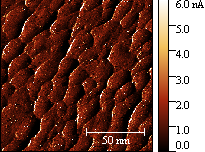
\includegraphics[width=\textwidth]{Bilder/Image01963_Strom.pdf}
        \caption{Strombild}
    \end{subfigure}
    \hspace{0.5cm}
    \begin{subfigure}{0.3\textwidth}
        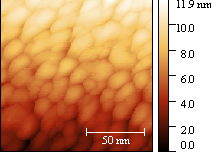
\includegraphics[width=\textwidth]{Bilder/Image01963_Rohdaten.pdf}
        \caption{Rohdaten Höhenbild}
    \end{subfigure}
    \hspace{0.5cm}
    \begin{subfigure}{0.3\textwidth}
        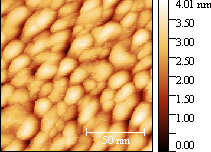
\includegraphics[width=\textwidth]{Bilder/Image01963_bearbeitet.pdf}
        \caption{Bearbeitetes Höhenbild}
    \end{subfigure}
    \caption{Bearbeitung der STM-Aufnahme einer Goldprobe mithilfe von Gwyddion. In der Mitte sind die importierten Rohdaten dargestellt. Rechts befindet sich das bearbeitete Höhenbild.}
    \label{fig:Bildbearbeitung}
\end{figure}
\subsection{Ablauf einer Messung}
Typischerweise ergibt sich bei einer Messaufnahme folgender Ablauf:
\begin{enumerate}
  \item Präparation der Spitze durch Schneiden mithilfe eines Seitenschneiders und anschließendes Platzieren im Scankopf
  \item Heranschieben des Piezoelements auf wenige Millimeter an die Spitze
  \item Motorgesteuertes manuelles Annähern der Probe mithilfe der Schaltfläche \textit{Advance} während die Probe durch eine Lupe beobachtet wird
  \item Durch Anklicken von \textit{Approach} wird die Probe nun vom Controller automatisch an die Spitze angenähert, bis ein Tunnelstrom von \SI{1}{\nano\ampere} fließt
  \item Wird die Spitze zum ersten Mal verwendet, sollte sie an einer bekannten Goldprobe getestet werden. Falls Spitzenfehler auftreten, können die durch Spitzenkonditionierung (Spannungspulse oder höhere Strome) behoben werden.
  \item Nun sollte das System bei gegebenen Parametern einige Zeit laufen, bis sich das Messsystem thermisch beruhigt hat. Anschließend kann die Messung gestartet werden.
\end{enumerate}
% *********************************************
% ***** KAPITEL 4 *****************************
% *********************************************
\newpage
\section{Ergebnisse und Diskussion}\label{sec:ErgebnisseUndDiskussion}
\subsection{Untersuchung der Goldprobe}
\subsubsection{Optimierung der Tunnelparameter}
Zunächst wurde versucht, durch Anpassung der verschiedenen Parameter in der Steuersoftware, ein möglich gutes Bild zu erhalten. Dafür wurde ein Scanbereich von $\SI{130}{\nano\metre} \times \SI{130}{\nano\metre}$ gewählt und die einzelnen Parameter variiert.
Die verfügbaren Parameter sind in folgender Tabelle zusammengefasst:
\begin{table}[ht]
	\centering
	\caption{Standardparameter für die STM-Aufnahme mithilfe der Steuersoftware Nanosurf easyScan}
	\label{tab:Parameter}
  \begin{tabular}{l c c c}
   \toprule
   Parameter   &       & Standardwert          & Wertebereich\\
   \midrule
   Setpoint    & $I$   & \SI{1}{\nano\ampere}  & $0.02-\SI{5}{\nano\ampere}$\\
   Tip Voltage & $U$   & \SI{1}{\volt}         & $-2 - \SI{2}{\volt}$\\
   P-Gain      & $K_P$ & 1000                  & 600-2000\\
   I-Gain      & $K_I$ & 500                   & 100-1500\\
   D-Gain      & $K_D$ & 0                     & \\
   Image Size  &       & \SI{130}{\nano\metre} & $4-\SI{512}{\nano\metre}$\\
   Time per Line &     & \SI{0.35}{\second}    & $0.052 - \SI{0.5}{\second}$\\
   Points per Line &   & 256                   &\\
   Rotation    &       & \SI{0}{\degree}       &\\ \bottomrule
  \end{tabular}
\end{table}
\paragraph{Optimierung des Tunnelstroms}$~$\\
Wie in Abschnitt \ref{sec:STM_Aufbau} bereits gezeigt wurde, entspricht ein aufgenommenes Bild konstanten Tunnelstroms einer Fläche konstanter Zustandsdichte. Zudem fällt der Tunnelstrom exponentiell mit steigendem Spitze-Probe Abstand ab. Wird nun die Spitze näher an die Probe herangeführt, fließt ein stärkerer Tunnelstrom und die Messung ergibt eine höhere Zustandsdichte. Werden nun bei einer STM Aufnahme die Tunnelströme variiert, ergibt sich das in Abbildung~\ref{fig:Stromvariation_1} gezeigte Bild.
\begin{figure}[htp]
    \centering
    \begin{subfigure}{0.45\textwidth}
        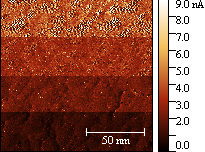
\includegraphics[height=4cm]{Bilder/Image01958_Stromvariation_Strom.pdf}
        \caption{Strombild}
    \end{subfigure}
    \hspace{0.5cm}
    \begin{subfigure}{0.45\textwidth}
        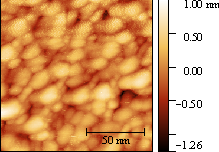
\includegraphics[height=4cm]{Bilder/Image01958_Stromvariation.pdf}
        \caption{Höhenbild}
    \end{subfigure}
    \caption{Variation des Setpoints $I$ innerhalb einer STM Aufnahme. Von unten nach oben wurde der Setpoint von $1 \text{ bis } \SI{4}{\nano\ampere}$ in gleichmäßigen Abständen variiert.}
    \label{fig:Stromvariation_1}
\end{figure}\\
Bei Erhöhung des Tunnelstroms zeigt sich eine leichte Verbesserung der Bildqualität, da durch den geringeren Abstand zwischen Probe und Spitze feine Details besser detektierbar sind. Wird die Stromstärke jedoch zu groß gewählt, tauchen deutliche Artefakte im Strombild auf, welche sich im Höhenbild niederschlagen. Zudem kann es bei diesen Strömen aufgrund der starken Wechselwirkung zwischen Spitze und Probe zur Umstruktuierung der Spitze kommen, was zur Zerstörung dieser führen kann. Jedoch kann ein hoher Tunnelstrom auch zur Konditionierung der Spitze verwendet werden, um eine Doppelspitze zu beheben. Weiterhin besteht bei einem höheren Tunnelstrom die Gefahr einer Kollision zwischen Probe und Spitze.\\
Wird der Tunnelstrom ausgehend vom Standardwert nach unten korrigiert lässt sich eine Verschmierung der Oberflächendetails beobachten (Abbildung~\ref{fig:Stromvariation_2}).
\begin{figure}[htp]
    \centering
    \begin{subfigure}{0.45\textwidth}
        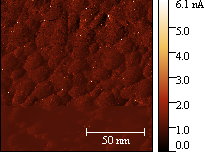
\includegraphics[height=4cm]{Bilder/Image01959_Stromvariation_Strom.pdf}
        \caption{Strombild}
    \end{subfigure}
    \hspace{0.5cm}
    \begin{subfigure}{0.45\textwidth}
        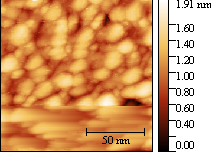
\includegraphics[height=4cm]{Bilder/Image01959_Stromvariation.pdf}
        \caption{Höhenbild}
    \end{subfigure}
    \caption{Variation des Setpoints $I$ innerhalb einer STM Aufnahme. Im oberen Drittel lag der Setpoint bei \SI{1}{\nano\ampere}, im mittlere Drittel bei \SI{0.5}{\nano\ampere} und im unteren Drittel bei \SI{0.05}{\nano\ampere}.}
    \label{fig:Stromvariation_2}
\end{figure}\\
Die Verschmierung wird verursacht durch den steigenden Einfluss der Zustandsdichte $\rho_\text{Spitze}$ der Tunnelspitze gegenüber der Zustandsdichte $\rho_\text{Probe}$ der Probe, da diese unabhängig vom Abstand zur Probe ist. Dadurch wird das Bild immer stärker durch die Struktur der Spitze beeinflusst und die Aufnahme verschmiert. Wird ein zu geringer Tunnelstrom (\SI{0.05}{\nano\ampere}) angelegt, dann besteht das Risiko, dass die Spitze den Kontakt zur Probe verliert. Es zeigt sich also, dass eine Variation des Tunnelstroms nach unten nicht sinnvoll ist.
\paragraph{Optimierung der Vorspannung}$~$\\
Zur weiteren Untersuchung der Tunnelparameter wird bei eingestellten Standardwerten die Spannung der Spitze (\textit{Tip Voltage}) innerhalb des Wertebereichs variiert. Wie in Abbildung~\ref{fig:Spannungsvariation} zu sehen ist, wurde die Spannung zwischen 1 bis \SI{2}{\volt} eingestellt.
\begin{figure}[htp]
    \centering
    \begin{subfigure}{0.45\textwidth}
        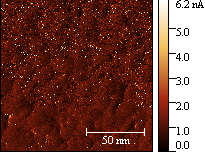
\includegraphics[height=4cm]{Bilder/Image01960_Spannungsvariation_Strom.pdf}
        \caption{Strombild}
    \end{subfigure}
    \hspace{0.5cm}
    \begin{subfigure}{0.45\textwidth}
        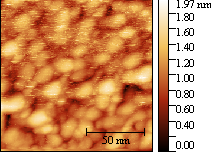
\includegraphics[height=4cm]{Bilder/Image01960_Spannungsvariation.pdf}
        \caption{Höhenbild}
    \end{subfigure}
    \caption{Variation \textit{Tip Voltage} zwischen \SI{2}{\volt} im oberen Drittel, \SI{1.5}{\volt} in der Mitte und \SI{1}{\volt} im unteren Drittel.}
    \label{fig:Spannungsvariation}
\end{figure}\\
Mithilfe von Formel~\eqref{eqn:Tunnelstrom} lässt sich der Einfluss der Vorspannung $U$ auf den Tunnelstrom beschreiben. Durch Erhöhung der Spannung muss zur Berechnung des Tunnelstroms über einen größeren Bereich integriert werden. Da der Integrand positiv ist, resultiert dies direkt in einer Erhöhung des Tunnelstroms. Somit treten die für die bereits bei Erhöhung des Tunnelstroms beobachteten Artefakte auch hier auf. Bei der Erhöhung des Tunnelstroms reagiert gleichzeitig auch der PID-Regelkreis und sorgt dafür, dass der Abstand zwischen Probe und Spitze erhöht wird, damit wieder ein konstanter Tunnelstrom herrscht. Es treten zusätzlich noch die für kleine Tunnelströme beobachteten Verschmierungen auf, was zeigt, dass eine Erhöhung der Vorspannung auf mehr als \SI{1}{\volt} für die Aufnahme von STM-Bildern nicht geeignet ist.\\
Allerdings ist es möglich durch kurzzeitige Erhöhung der Spannung mithilfe eines Spannungspulses die Spitze zu konditionieren und eine Doppelspitze zu beheben. In der \textit{Nanosurf easyScan} Steuersoftware gibt es dafür die Schaltfläche \textit{Tip Cleaning Pulse}.\\
Es sollte in allen Fällen vermieden werden, bei der Variation von $U$ eine Spannung von \SI{0}{\volt} einzustellen. Wenn dies geschieht, fließt kein Tunnelstrom mehr und der PID-Regelkreis steuert die Spitze zur Erhöhung des Tunnelstroms in die Probe hinein und die Spitze wird beschädigt. Weiterhin treten Probleme auf, wenn negative Spannungen verwendet werden. Theoretisch sollte sich beim Vorzeichenwechsel der Spannung die Richtung des Tunnelstroms ändern, jedoch trat im Experiment bei negativen Spannungen ein Kontaktverlust zwischen Probe und Spitze auf, was bei einer erneuten Annäherung zur Probe zu einer Kollision führte. Aus diesem Grund wird im Folgenden auf die Verwendung von negativen Spannungen verzichtet.
\paragraph{Optimierung der Regelparameter}$~$\\
Im weiteren Verlauf findet eine Optimierung der drei Regelparameter statt, damit die Oberfläche mit einer geeigneten Geschwindigkeit abgetastet wird. Aufgrund der endlichen Regelzeit, kann der PID-Regler nicht instantan auf Änderungen der Zustandsdichte reagieren, weshalb scharfe Kanten verschmieren. Das generelle Ziel ist es, eine möglichst scharfes Höhenbild ohne Artefakte zu erzeugen. Das Strombild zeigt im Idealfall eine homogene Struktur und gibt Aufschluss über die Effektivität der Regelung. Sind im Strombild Strukturen zu erkennen, dann sollte die Regelung angepasst werden.\\
Zunächst wurde der Faktor $K_P$ des Proportionalgliedes verändert (siehe Abbildung~\ref{fig:PGlied}).
\begin{figure}[htp]
    \centering
    \begin{subfigure}{0.45\textwidth}
        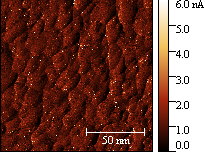
\includegraphics[height=4cm]{Bilder/Image01979_PGain_Strom.pdf}
        \caption{Strombild}
    \end{subfigure}
    \hspace{0.5cm}
    \begin{subfigure}{0.45\textwidth}
        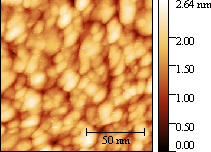
\includegraphics[height=4cm]{Bilder/Image01979_PGain.pdf}
        \caption{Höhenbild}
    \end{subfigure}
    \caption{Variation von $K_P$ von oben nach unten mit $K_P = 1000, 1500, 2000, 600$}
    \label{fig:PGlied}
\end{figure}\\
In dem aufgenommen Bild zeigt sich keine große Abweichung bei der Änderung des P-Gain Parameters $K_P$.\\
Theoretisch sorgt ein größerer Werte von $K_P$ für die Ausbildung einer Schwingung des Regelkreises, welche zur Aufweichung von Kanten führt. Wird die Regelgröße zu groß gewählt, kann sich eine Überschwingung ausbilden, was das Risiko der Spitzenkollision birgt. Jedoch zeigt sich, dass diese Schwingungen für die verwendeten Parameter (innerhalb des empfohlenen Wertebereichs) nicht signifikant genug auftreten, um die Bildqualität zu beeinträchtigen.\\

Als zweites wurde der Einfluss des $K_I$ Parameters auf die Messung untersucht. Dafür wurde der I-Gain ausgehend von den Standardwerten nach oben und unten variiert und in Abbildung~\ref{fig:IGlied} dargestellt.
\begin{figure}[htp]
    \centering
    \begin{subfigure}{0.45\textwidth}
        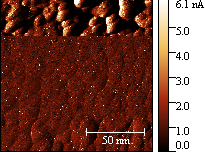
\includegraphics[height=4cm]{Bilder/Image01980_IGain_Strom.pdf}
        \caption{Strombild}
    \end{subfigure}
    \hspace{0.5cm}
    \begin{subfigure}{0.45\textwidth}
        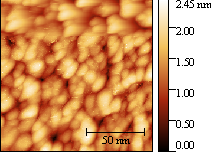
\includegraphics[height=4cm]{Bilder/Image01980_IGain.pdf}
        \caption{Höhenbild}
    \end{subfigure}
    \caption{Variation von $K_I$ von unten nach oben mit $K_I = 500, 1000, 1500, 100$}
    \label{fig:IGlied}
\end{figure}\\
Im Höhenbild ist erkennbar, dass die Schärfe des Bildes für steigende Werte des Parameters $K_I$ zunimmt. Dies lässt sich dadurch erklären, dass die Regelung für kleine Werte träge wird. Im Strombild ist dies dadurch erkennbar, dass dort die Struktur der Probe auftaucht. Da die Information des Bildes nun auf Strom- und Höhenbild verteilt wird, tritt eine Verschlechterung des Höhenbildes auf und es erscheint verschmiert. Für zu hohe Werte treten allerdings wieder Artefakte auf, was auf den durch die Regelung kurzzeitigen hohen Tunnelstrom zurückzuführen ist.\\
Da der I-Regler durch die Summation der Regelung langanhaltene Veränderungen der Stellgröße registiert, werden niedrige Frequenzen verstärkt, was auf ein Tiefpassverhalten schließen lässt.\\
Der differentielle Parameter $K_D$ wird standardmäßig auf Null gesetzt wird in dieser Messung nicht varriert, denn er verstärkt aufgrund seines intensiven Regelverhaltens für schnelle Veränderungen das Auftreten von Artefakten und zeigt damit ein Hochpassverhalten.
\paragraph{Optimierung der Abtastgeschwindigkeit}
Zur besseren Analyse der Abtastgeschwindigkeit wurde zur Aufnahme der Bilder die Auflösung heraufgesetzt auf 512 Messpunkte pro Linie, um Unterschiede besser erkennen zu können.
Es wurde nun während der Aufnahme die Abtastgeschwindigkeit von \SI{0.4}{\second\per\text{Line}} auf \SI{0.8}{\second\per\text{Line}} erhöht (siehe Abbildung~\ref{fig:Abtastgeschwindigkeit}).
\begin{figure}[htp]
    \centering
    \begin{subfigure}{0.45\textwidth}
        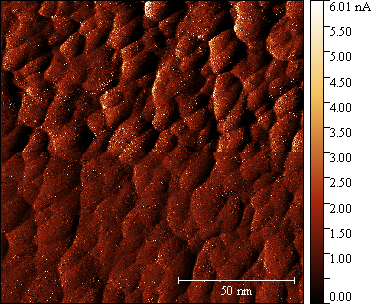
\includegraphics[height=4cm]{Bilder/Image01982_ppl512_Strom.pdf}
        \caption{Strombild}
    \end{subfigure}
    \hspace{0.5cm}
    \begin{subfigure}{0.45\textwidth}
        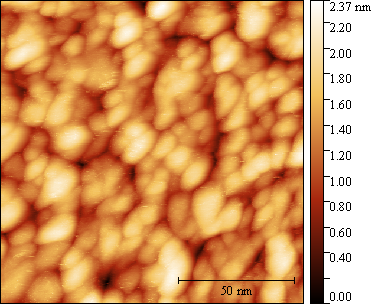
\includegraphics[height=4cm]{Bilder/Image01982_ppl512.pdf}
        \caption{Höhenbild}
    \end{subfigure}
    \caption{Änderung der Abtastgeschwindigkeit pro Zeile von oben nach unten: \SI{0,4}{\second\per\text{Line}}, \SI{0.8}{\second\per\text{Line}}}
    \label{fig:Abtastgeschwindigkeit}
\end{figure}\\
Zunächst wird die Abbildung aufgrund der höheren Bildauflösung schärfer. Weiterhin ist erkennbar, dass für eine langsamere Abtastgeschwindigkeit im unteren Teil des Strombildes die Struktur nicht mehr so gut erkennbar ist, was zu einer Verbesserung des Höhenbildes führt. Dieses zeigt zusätzlich in der unteren Bildhälfte weniger Artefakte. Die kleinere Abtastgeschwindigkeit lässt dem Regelkreis mehr Zeit, die Höhe der Spitze anzupassen und das Strombild wird homogener. Allerdings ist diese Methode zeitaufwändig und nicht praktikabel, wenn der Einfluss des thermischen Drifts sehr hoch ist (siehe Graphenprobe).\\

Zusammenfassend ergeben sich nun folgende angepasste Parametergrößen:
\begin{table}[ht]
	\centering
	\caption{Anpassung der Parameter}
	\label{tab:Parameteranpassung}
  \begin{tabular}{c c c c c c}
   \toprule
   Setpoint & Tip Voltage & P-Gain & I-Gain & D-Gain & time/Line\\
   \midrule
   \SI{1}{\nano\ampere} & \SI{0.5}{\volt} & 1500 & 1000 & 0 & \SI{0.35}{\second\per\text{Line}}\\
   \bottomrule
  \end{tabular}
\end{table}\\
Allerdings ist die Anpassung der Parameter auch abhängig von der Beschaffenheit der Probe, weshalb die Parameter für andere Proben individuell angepasst wurden.

\subsubsection{Probenaufnahme und thermischer Drift}
Zur Überprüfung der aufgenommen Probe auf das Vorliegen einer Doppelspitze oder anderen Artefakten wurde das Bild in verschiedenen Größen aufgenommen, um eventuell auftauchende periodische Strukturen auszuschließen.
Für die einzelnen Bildausschnitte wurde jeweils die Abtastgeschwindigkeit pro Linie angepasst, damit kein Qualitätsverlust auftritt. Die Ergebnisse zeigt Abbildung~\ref{fig:verschiedeneGroesse}.
\begin{figure}[htp]
    \centering
    \begin{subfigure}{0.3\textwidth}
        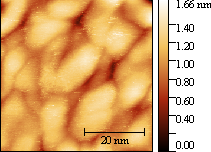
\includegraphics[width=\textwidth]{Bilder/Image01989_50nm.pdf}
        \caption{$\SI{50}{\nano\metre}\times\SI{50}{\nano\metre}$}
    \end{subfigure}
    \hspace{0.5cm}
    \begin{subfigure}{0.3\textwidth}
        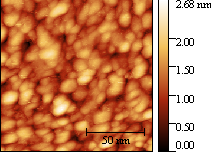
\includegraphics[width=\textwidth]{Bilder/Image01985_130nm.pdf}
        \caption{$\SI{130}{\nano\metre}\times\SI{130}{\nano\metre}$}
    \end{subfigure}
    \hspace{0.5cm}
    \begin{subfigure}{0.3\textwidth}
        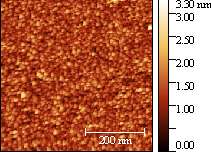
\includegraphics[width=\textwidth]{Bilder/Image01986_512nm.pdf}
        \caption{$\SI{512}{\nano\metre}\times\SI{512}{\nano\metre}$}
    \end{subfigure}
    \caption{Aufnahme der Probe in verschiedenen Größen. Dabei wurde die Abtastgeschwindigkeit entsprechend zwischen \SI{0,3}{\second\per\text{Line}} bis \SI{0,5}{\second\per\text{Line}} variiert.}
    \label{fig:verschiedeneGroesse}
\end{figure}\\
Bei einigen Aufnahmen ließ sich ein besonderes Phänomen beobachten. Das Programm \textit{Nanosurf easyScan} Steuersoftware, scannt den Bereich immer abwechselnd von oben nach unten und vice versa. Dabei erschienen die einzelnen Goldatome manchmal tropfenförmig verzerrt, während sie in der zweiten Aufnahme normal erscheinen. Zwei Beispielaufnahmen dazu sind im folgenden Bild~\ref{fig:ThermischerDrift} dargestellt.
\begin{figure}[htp]
    \centering
    \begin{subfigure}{0.45\textwidth}
        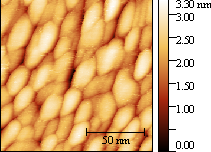
\includegraphics[height=4cm]{Bilder/Image01966_Drift_obenunten.pdf}
        \caption{Abtastung von oben nach unten}
    \end{subfigure}
    \hspace{0.5cm}
    \begin{subfigure}{0.45\textwidth}
        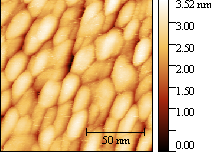
\includegraphics[height=4cm]{Bilder/Image01965_Drift_untenoben.pdf}
        \caption{Abtastung von unten nach oben}
    \end{subfigure}
    \caption{Veranschaulichung des thermischen Drifts der Goldprobe bei Abtastung des gleichen Ausschnitts entlang und entgegen des thermischen Drifts.}
    \label{fig:ThermischerDrift}
\end{figure}\\
Dieser Bildfehler wird durch den thermischen Drift verursacht, welcher durch die unterschiedliche thermische Ausdehnung von Probe und Tunnelspitze infolge des Tunnelstroms auftritt. Zudem können Schwankungen der Raumtemperatur den thermischen Drift beeinflussen.\\
Wird nun die Probe entlang des thermischen Drifts abgerastert erscheinen die Atome länglich verzerrt, findet die Abrasterung entgegen des Drifts statt, werden die Atome gestaucht. Es sollten bei Möglichkeit immer zwei Aufnahme der Probe gemacht werden, um Einflüsse des thermischen Drifts auszuschließen.\\
Im Verlauf der Messung wird der Effekt des thermischen Drifts geringer. In der Praxis wird die Probe gekühlt, um thermische Effekte zu minimieren.

\subsubsection{Charakterisierung der Probenoberfläche}
Zur Charakterisierung der Goldoberfläche wurde eine Aufnahme der Goldprobe von $\SI{130}{\nano\metre}\times\SI{130}{\nano\metre}$ verwendet. Diese zeigt eine gute Bildqualität zur Auswertung von der Rauheit und den Korngrößen.\\
Zunächst wurde mithilfe von Gwyddion ein Höhenprofil extrahiert, welches in Abbildung~\ref{fig:HoehenprofilGold} gezeigt wird.
\begin{figure}[htp]
    \centering
    \begin{subfigure}{0.45\textwidth}
        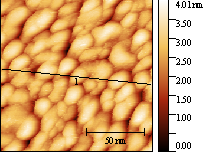
\includegraphics[height=4cm]{Bilder/Image01963_Bild_Hoehenprofil.pdf}
        \caption{Verwendetes Bild zur Erstellung der Höhenlinie}
    \end{subfigure}
    \hspace{0.5cm}
    \begin{subfigure}{0.45\textwidth}
        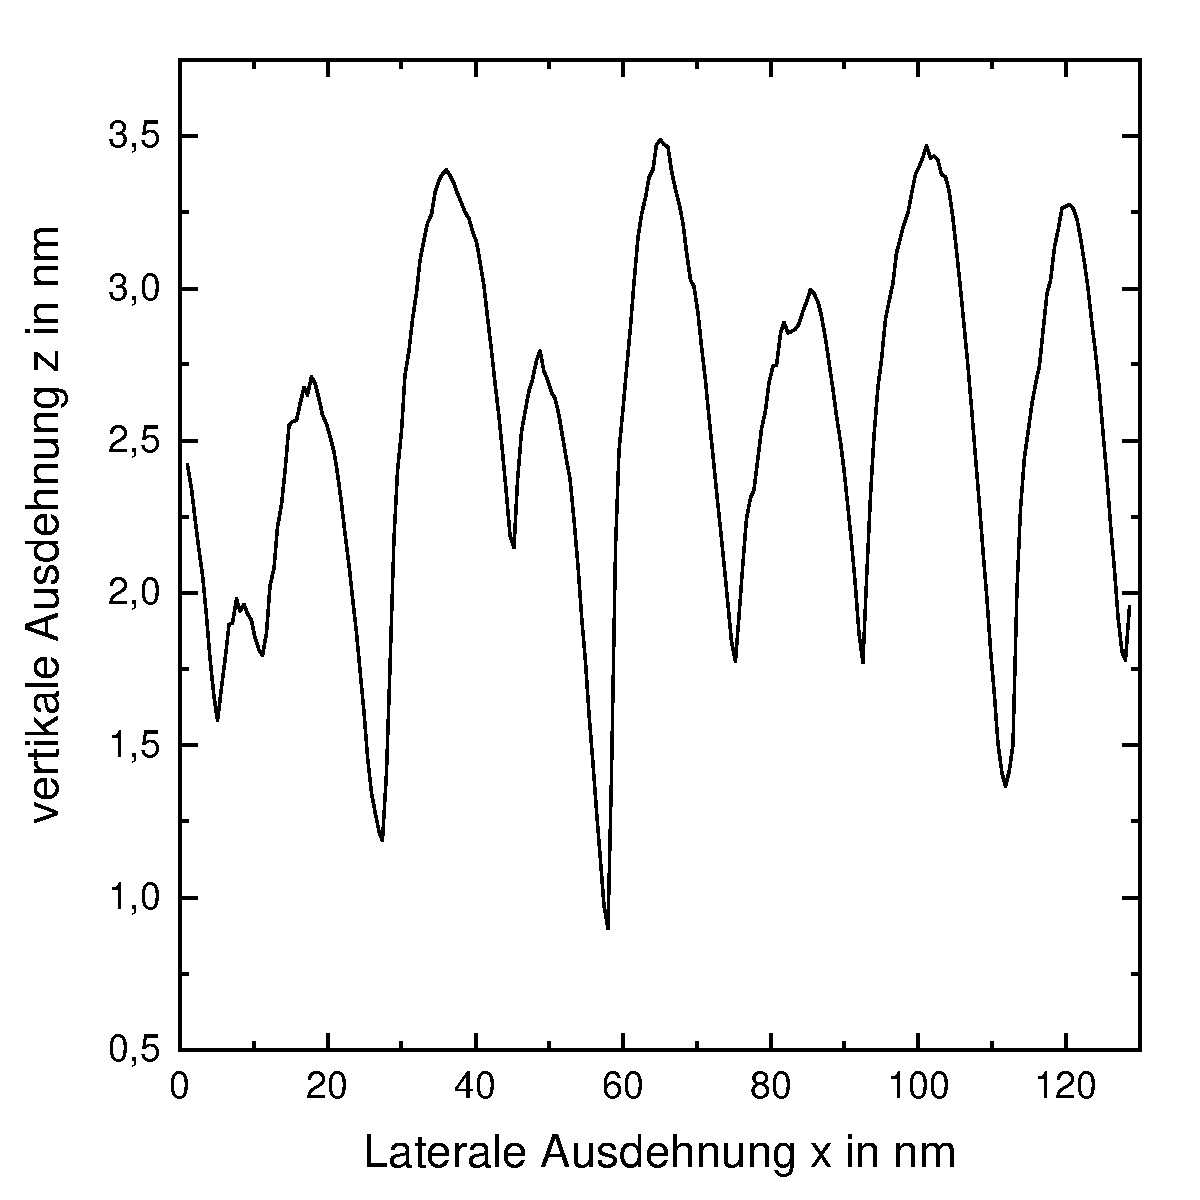
\includegraphics[height=4cm]{Bilder/Image01963_Hoehenprofil.pdf}
        \caption{Höhenlinie der Goldprobe\\}
    \end{subfigure}
    \caption{Mithilfe von Gwyddion wurde ein Höhenprofil des aufgenommen Bildes der Goldprobe erstellt. In a) ist die Linie eingezeichnet, entlang derer das Höhenprofil aufgenommen wurde.}
    \label{fig:HoehenprofilGold}
\end{figure}\\
Es ergibt sich eine unregelmäßige Struktur, mit Korngrößen zwischen 10 und \SI{20}{\nano\metre}, mit maximalen Höhenunterschieden von \SI{2.5}{\nano\metre}.\\
Um nun die Körnung der Oberfläche statistisch auszuwerten, muss zunächst eine Maskierung der Körner durchgeführt werden. Dafür bietet Gwyddion verschiedene Tools an. Eine rein durch einen Schwellwert basierende Maskierung lieferte ungenügend gute Ergebnisse, weshalb der \textit{Watershed} Algorithmus (zu deutsch: Wasserscheidentransformation) verwendet wurde.~\cite{Gwyddion_documentation} In diesem zweistufigen Algorithmus werden die Körner zunächst lokalisiert und anschließend zusammenhängende Körner segmentiert. Dabei kann zudem ein Schwellwert für die Korngröße eingestellt werden. Die resultierende Maskierung zeigt Abbildung~\ref{fig:Kornflaechen}
\begin{figure}[htp]
    \centering
    \begin{subfigure}{0.45\textwidth}
        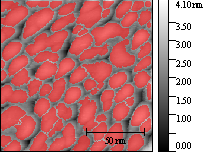
\includegraphics[height=4cm]{Bilder/Image01963_Korngroessen.pdf}
        \caption{Maskierung der Körner}
    \end{subfigure}
    \hspace{0.5cm}
    \begin{subfigure}{0.45\textwidth}
        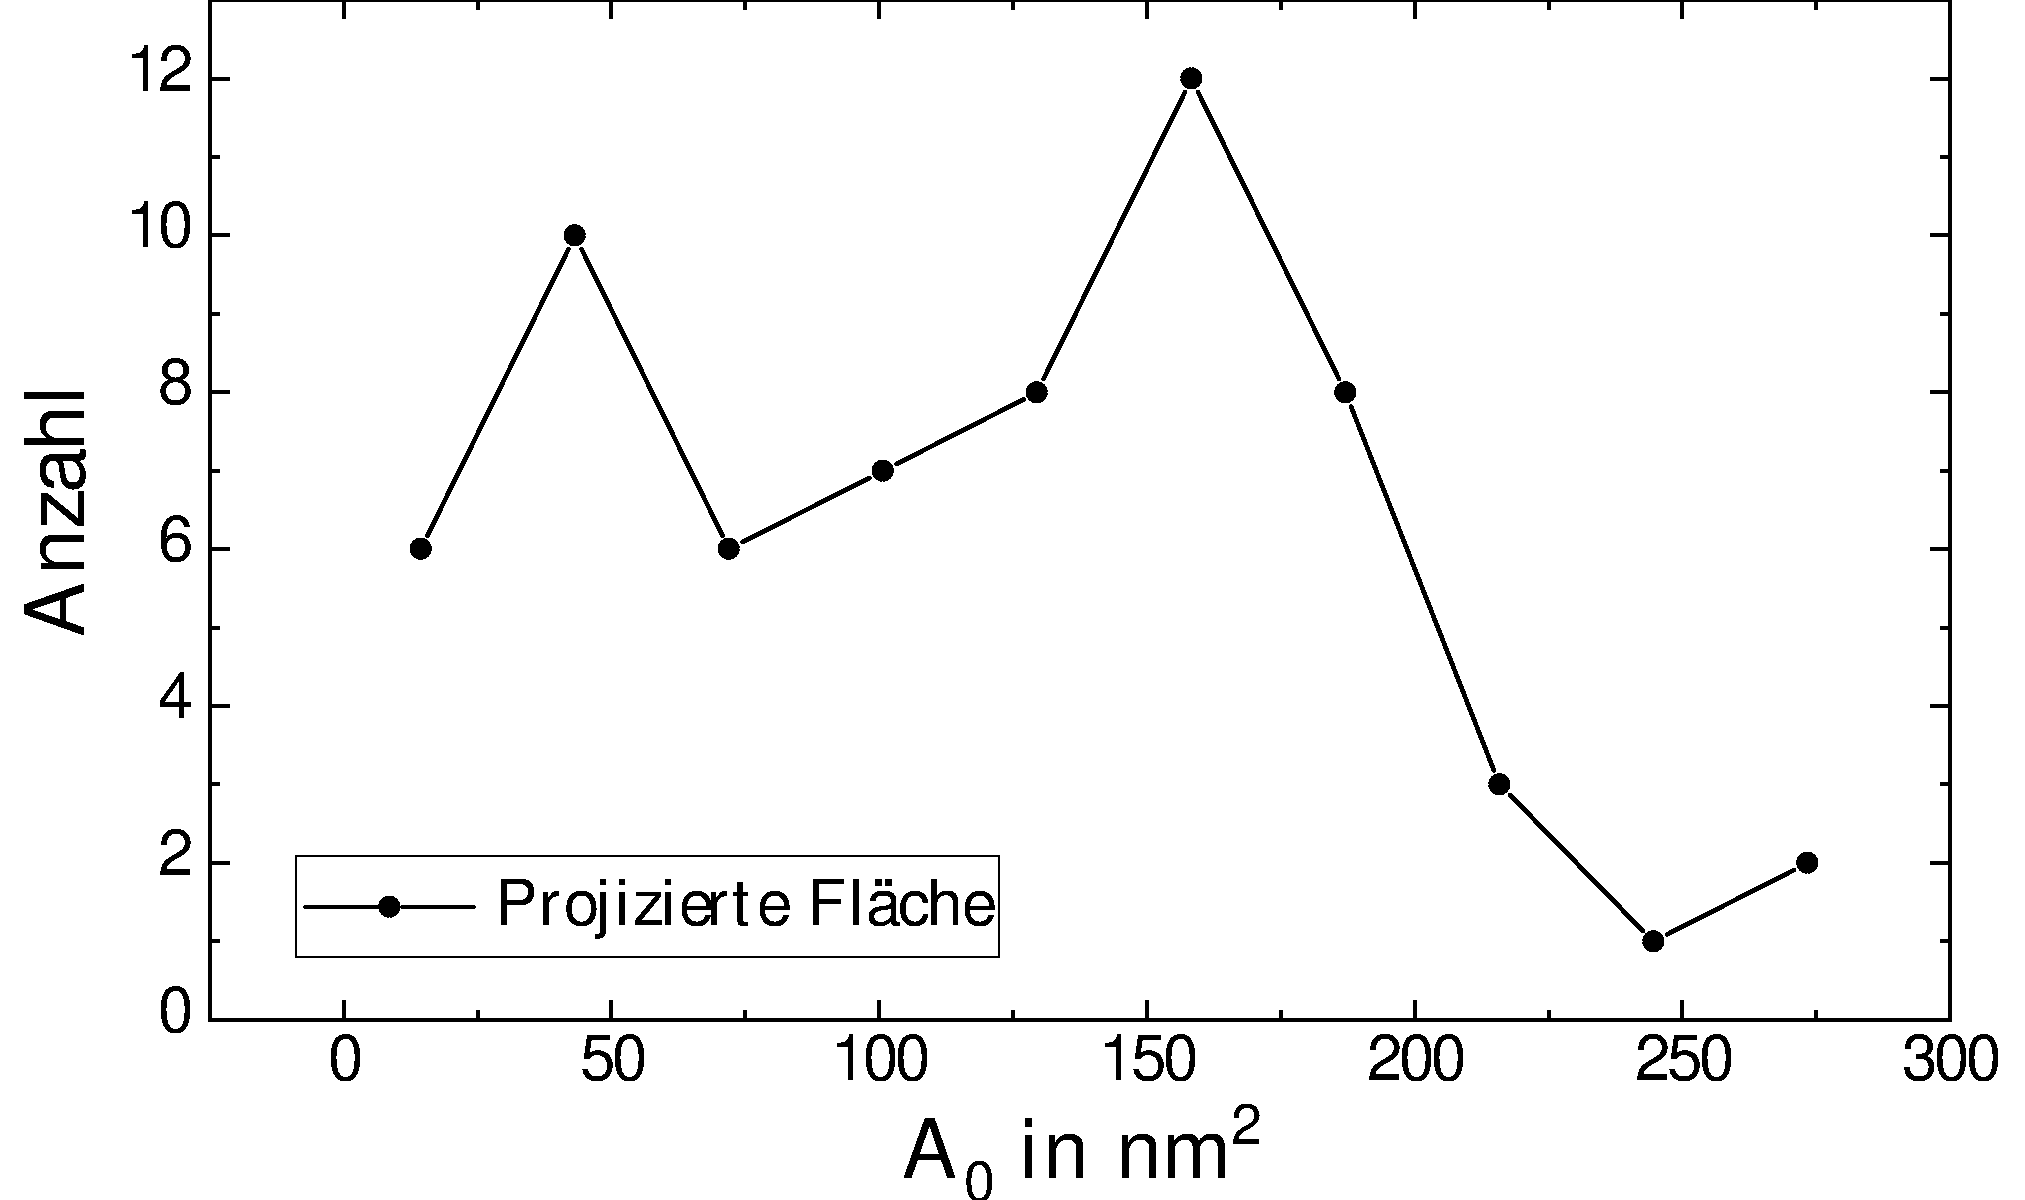
\includegraphics[height=4cm]{Bilder/Image01963_ProjizierteFlaeche.pdf}
        \caption{Projizierte Kornfläche}
    \end{subfigure}
    \caption{Anwendung des Watershed Algorithmus auf die Körner. Es wurden folgende Parameter verwendet: Korn-Lokalisierung in 15 Schritten, Tropfengröße \SI{7}{\percent}, Schwellwert \SI{68}{\text{px}\squared}, Segmentierung in 100 Schritten, Tropfengröße, \SI{5}{\percent}}
    \label{fig:Kornflaechen}
\end{figure}\\
Mithilfe der Maskierung können nur durch Gwyddion durch statistische Auswertung verschiedene Charakteristika der Probe ausgemessen werden. In Abbildung~\ref{fig:Kornflaechen} b) ist die Verteilung der projizierten Kornflächen dargestellt. Es zeigt sich eine Häufung der Korngrößen bei einer Fläche von \SI{50}{\nano\metre\squared} und \SI{150}{\nano\metre\squared}.\\
Zur Angabe der Rauheit einer Oberfläche eignen sich verschiedene Rauheitsangaben. Die mittlere Rauheit $R_a$ gibt den mittleren Abstand zur Mittellinie des Höhenprofils an~\cite{Rauheit}. Er entspricht dem arithmetischen Mittel der betragsmäßigen Abweichung vom Mittelwert. Für ein quadratisches Bild ergibt sich:
\begin{align}
  R_a = \frac{1}{N^2} \sum_{m,n = 1}^N |z(x_m, x_n) - \langle z \rangle|,
\end{align}
wobei der Mittelwert $\langle z \rangle$ folgendermaßen gegeben ist:
\begin{align}
  \langle z \rangle \frac{1}{N^2} \sum_{m,n = 1}^N z(x_m, y_n).
\end{align}
Andererseits lässt sich die quadratische Rauheit RMS (\textit{root-mean-squared roughness}) angeben als Wurzel des Mittels der Abweichungsquadrate~\cite{Rauheit}.
Der RMS Wert entspricht also dem quadratischen Mittel:
\begin{align}
  \text{RMS} = \sqrt{\frac{1}{N^2}\sum_{m,n = 1}^N (z(x_m, y_n)-\langle z\rangle)^2}.
\end{align}
Die einzelnen Rauhigkeitswerte können in Gwyddion direkt in den Statistiken zur Korngröße abgelesen werden und sind in Tabelle~\ref{tab:ErgebnisseGoldprobe} zusammengefasst.
\begin{table}[ht]
	\centering
	\caption{Ergebnisse der statistischen Auswertung der Probe}
	\label{tab:ErgebnisseGoldprobe}
  \begin{tabular}{c c c c}
   \toprule
   Größe & Wert & Größe & Wert\\
   \midrule
   Kornanzahl & 72 & Mittlere Kornfläche & \SI{149}{\nano\metre\squared}\\
   Rauhigkeit RMS & \SI{245}{\pico\metre} & Mittlere Korngröße & \SI{11.4}{\nano\metre}\\
   \bottomrule
  \end{tabular}
\end{table}\\
%%%%%%%%%%%%%%%%%%%%%%%%%%%%%%%%%%%%%%%

% *********************************************
% ***** KAPITEL 5 *****************************
% *********************************************
\section{Zusammenfassung}
%%%%%%%%%%%%%%%%%%%%%%%%%%%%%%%%%%%
% ***** Literaturverzeichnis ******************

\begin{thebibliography}{xxx}
\bibitem{Hamann}
C. Hamann und M. Hietschold: \textit{Raster-Tunnel-Mikroskopie}. Akademie Verlag GmbH, Berlin 1991.
\bibitem{Mayer}
D. Bonnell: \textit{Scanning Tunneling Microscopy and Spectroskopy}. VCH Publishers, Inc. 1993.
\bibitem{Versuchsanleitung}
M. Grünewald: \textit{FSU Fortgeschrittenenen Praktikum: SPM}. Fried\-rich-Schil\-ler-Uni\-versi\-tät Jena, Mai 2019.
\bibitem{Demtroeder}
W. Demtroeder: \textit{Experimentalphysik 3: Atome, Moleküle und Festkörper}. Springer-Verlag Berlin Heidelberg 2016 (5. Auflage).
\bibitem{Nanosurf}
Nanosurf AG: \textit{easyScan 2 STM: Operating Instructions}. Liestal 2009.
\bibitem{Gwyddion}
D. Nečas und P. Klapetek: \textit{Gwyddion: Free SPM (AFM, SNOM/NSOM, STM, MFM, $\hdots$), data analysis software}. Version 2.55, \url{gwyddion.net}, (Stand: 17.01.2020).
\bibitem{Gwyddion_documentation}
D. Nečas, P. Klapetek, Christopher Anderson: \textit{Gwyddion user guide}, \url{http://gwyddion.net/documentation/user-guide-en/index.html}, (Stand: 20.01.2020)
\bibitem{Forker}
R. Forker: \textit{Tutorial zum Messtechnikpraktikum: Versuch 5, PID-Regler}. Fried\-rich-Schil\-ler-Uni\-versi\-tät Jena, 2019.
\bibitem{Rauheit}
URL: \url{https://de.wikipedia.org/wiki/Rauheit}, (Stand: 20.01.2020)
\end{thebibliography}
\end{document}
